\documentclass[tikz]{standalone}
\usepackage[permutation,huge,neon]{causets}
\usetikzlibrary{fit,shapes.geometric}
\begin{document}
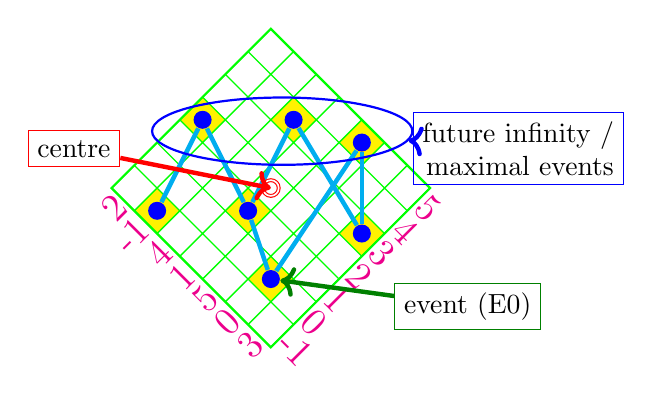
\begin{tikzpicture}
	% Create causet, shifted in x- and y-direction:
	\begin{scope}[xshift=3cm, yshift=-1cm]
		\tikzcausetsset{offset=-2}
		\drawpcauset{5,2,7,3,6,1,4}
		\draw[red, double] (0, 0) circle[radius=0.1];
	\end{scope}
	% Circumscribe the future infinity:
	\node[draw=blue, inner sep=1pt, thick, ellipse, fit=(E2) (E4) (E5)] (Finf) {};
	% Add labels on top:
	\node[draw=blue, right, align=right] (FinfLabel) at (4.8, -0.5) {future infinity / \\ maximal events};
	\node[draw=red] (centerLabel) at (0.5, -0.5) {centre};
	\node[draw=green!50!black] (myEventLabel) at (5.5, -2.5) {event (E0)};
	% Draw arrows from the labels to the references:
	\draw[ultra thick, blue, ->] (FinfLabel) -- (Finf);
	\draw[ultra thick, red, ->] (centerLabel) -- (3, -1);
	\draw[ultra thick, green!50!black, ->] (myEventLabel) -- (E0);
\end{tikzpicture}
\end{document}
